Administrarea utilizatorilor este foarte importanta, orice aplicatie
este construita pentru utilizatorii sai. Elementele necesare in cazul
specific al RODA sunt cele clasice: posibilitatea trecerii in revista
a utilizatorilor sistemului, posibilitatea invalidarii acestora daca
este cazul, posibilitatea asocierii acestora la diferite grupuri pentru
a li se atribui diferite seturi de drepturi, posibilitatea modificarii
datelor personale ale acestora in cazul in care este nevoie, etc. 

RODA nu va avea (si nu are nevoie) de un sistem avansat de interactiune
sociala intre utilizatori, acestia nu trebuie sa se poata invita unii
pe ceilalti sa faca parte din diferite grupuri si nici nu vor avea
liste de prieteni sau alt fel de asocieri arbitrare. 

Administrarea utilizatorilor se va face intr-un ecran dedicat, de
unde vor fi accesibile toate operatiile necesare. 

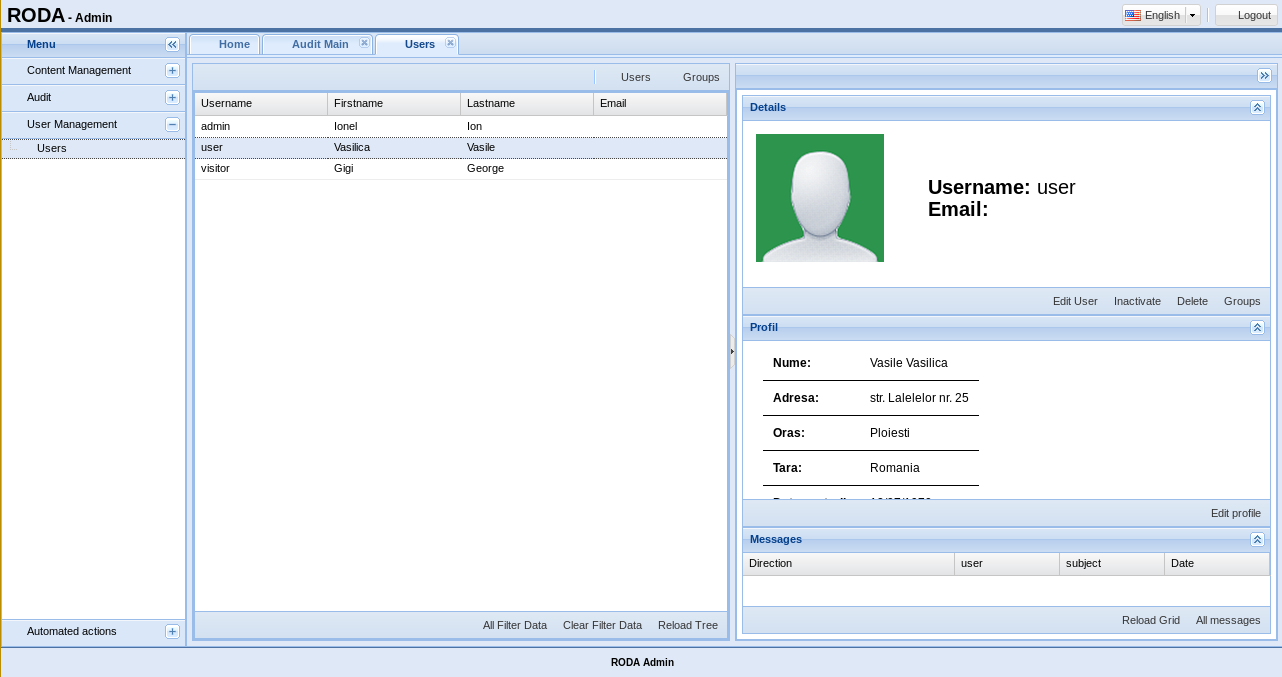
\includegraphics[width=15cm]{user/user1}

Zona de detalii este impartita in trei segmente - unul care contine
informatiile fundamentale ale utilizatorului (nume, email, etc.),
una care contine informatiile de profil ale acestuia (adresa, data
nasterii) si una care contine lista de mesaje pe care acesta le-a
primit de la sistem sau de la administratori. 

Mesajele trimise utilizatorilor de catre sistem sau de catre administratori
sunt importante - ele contin informatii pe care utilizatorul trebuie
sa le stie. Este important pentru administratori sa stie daca un anumit
utilizator cunoaste aceste informatii, pentru a rezolva eventuale
probleme pe care acesta le poate avea in utilizarea sistemului.

Ca lista de utilizatori, administratorii pot apela din ecranul din
partea stanga si lista de grupuri. 

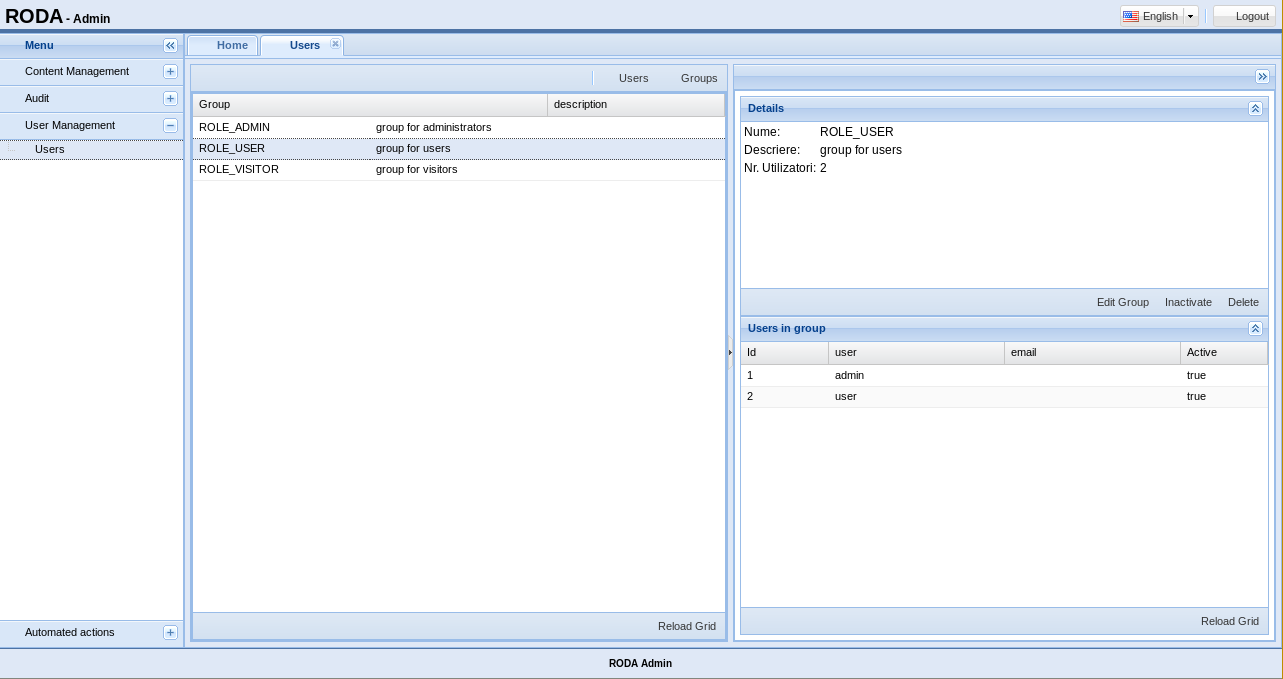
\includegraphics[width=15cm]{user/user4}

Detaliile disponibile in cazul unui grup sunt mai putine - numele
si descrierea acestuia precum si lista utilizatorilor care fac parte
din grupul curent. 

Modulul permite de asemenea adaugarea sau modificarea utilizatorilor:

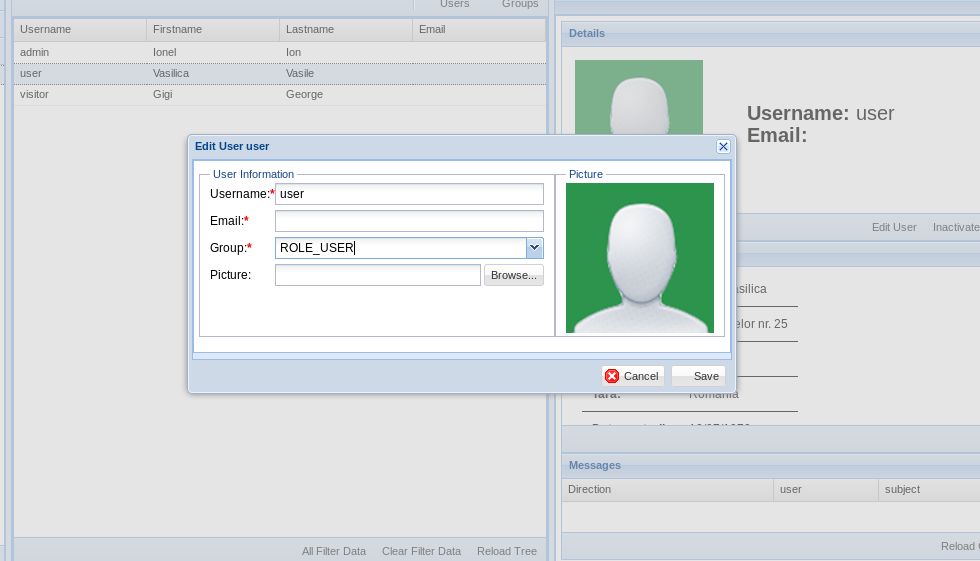
\includegraphics[width=10cm]{user/user2}

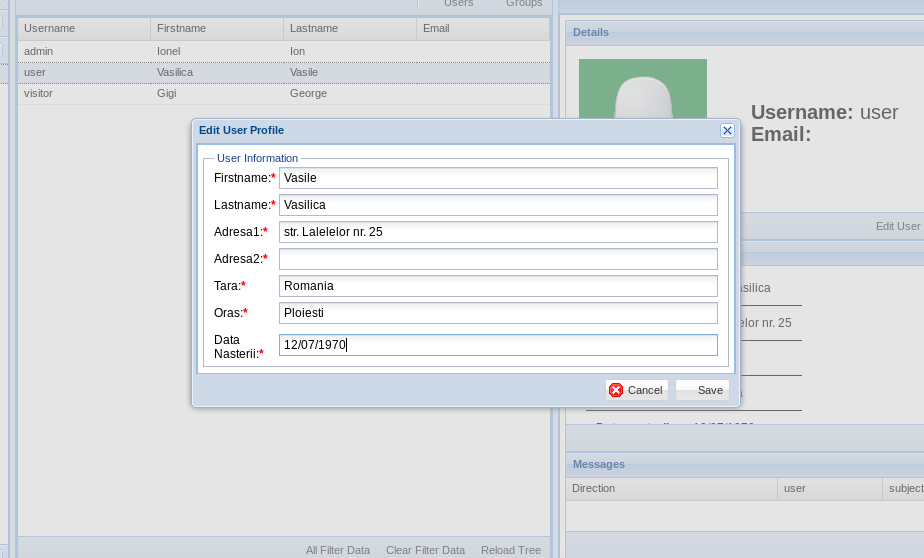
\includegraphics[width=10cm]{user/user3}

Modulul permite de asemenea modificarea proprietatilor grupurilor.

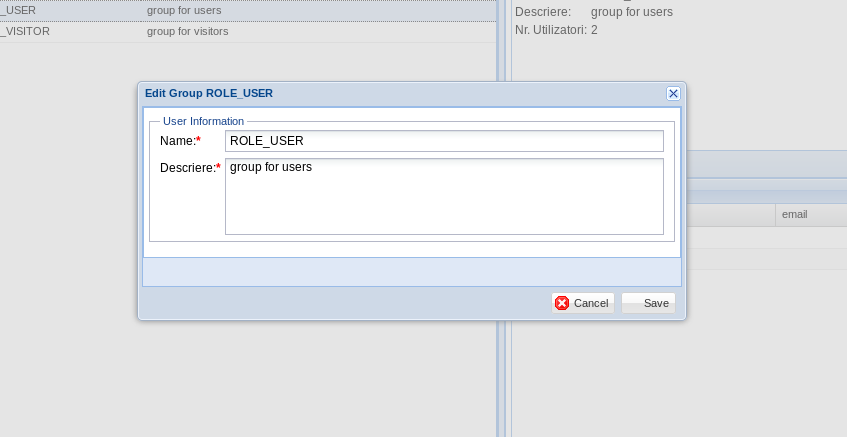
\includegraphics[width=10cm]{user/user5}
